\documentclass[
11pt, % The default document font size, options: 10pt, 11pt, 12pt
%codirector, % Uncomment to add a codirector to the title page
]{charter} 
% El títulos de la memoria, se usa en la carátula y se puede usar el cualquier lugar del documento con el comando \ttitle
\titulo{Desarrollo de aplicación Hospitalaria con MQTT} 

% Nombre del posgrado, se usa en la carátula y se puede usar el cualquier lugar del documento con el comando \degreename
%\posgrado{Carrera de Especialización en Sistemas Embebidos} 
\posgrado{Carrera de Especialización en Internet de las Cosas} 
%\posgrado{Carrera de Especialización en Intelegencia Artificial}
%\posgrado{Maestría en Sistemas Embebidos} 
%\posgrado{Maestría en Internet de las cosas}

% Tu nombre, se puede usar el cualquier lugar del documento con el comando \authorname
\autor{Ing. Gustavo Bastian} 

% El nombre del director y co-director, se puede usar el cualquier lugar del documento con el comando \supname y \cosupname y \pertesupname y \pertecosupname
\director{Mg.Ing. Ericson Joseph Estupiñan Pineda}
\pertenenciaDirector{Surix S.R.L} 
% FIXME:NO IMPLEMENTADO EL CODIRECTOR ni su pertenencia
%\codirector{John Doe} % para que aparezca en la portada se debe descomentar la opción codirector en el documentclass
%\pertenenciaCoDirector{FIUBA}

% Nombre del cliente, quien va a aprobar los resultados del proyecto, se puede usar con el comando \clientename y \empclientename
\cliente{Ing. Sergio Starkloff}
\empresaCliente{Surix S.R.L}

% Nombre y pertenencia de los jurados, se pueden usar el cualquier lugar del documento con el comando \jurunoname, \jurdosname y \jurtresname y \perteunoname, \pertedosname y \pertetresname.
\juradoUno{Nombre y Apellido (1)}
\pertenenciaJurUno{pertenencia (1)} 
\juradoDos{Nombre y Apellido (2)}
\pertenenciaJurDos{pertenencia (2)}
\juradoTres{Nombre y Apellido (3)}
\pertenenciaJurTres{pertenencia (3)}
 
\fechaINICIO{31 de Octubre de 2021}		%Fecha de inicio de la cursada de GdP \fechaInicioName
\fechaFINALPlan{7 de Diciembre de 2021} 	%Fecha de final de cursada de GdP
\fechaFINALTrabajo{15 de mayo de 2022}	%Fecha de defensa pública del trabajo final


\begin{document}

\maketitle
\thispagestyle{empty}
\pagebreak


\thispagestyle{empty}
{\setlength{\parskip}{0pt}
\tableofcontents{}
}
\pagebreak


\section*{Registros de cambios}
\label{sec:registro}


\begin{table}[ht]
\label{tab:registro}
\centering
\begin{tabularx}{\linewidth}{@{}|c|X|c|@{}}
\hline
\rowcolor[HTML]{C0C0C0} 
Revisión & \multicolumn{1}{c|}{\cellcolor[HTML]{C0C0C0}Detalles de los cambios realizados} & Fecha      \\ \hline
0      & Creación del documento                                 & 31/10/2021 \\ \hline
1      & Se completa hasta el punto 5 inclusive                 & 3/11/2021 \\ \hline
2      & Se completa hasta el punto 9 inclusive
& 11/11/2021 \\ \hline
%		  Se puede agregar algo más \newline
%		  En distintas líneas \newline
%		  Así                                                    & dd/mm/aaaa \\ \hline
%3      & Se completa hasta el punto 11 inclusive                & dd/mm/aaaa \\ \hline
%4      & Se completa el plan	                                 & dd/mm/aaaa \\ \hline
\end{tabularx}
\end{table}

\pagebreak



\section*{Acta de constitución del proyecto}
\label{sec:acta}

\begin{flushright}
Buenos Aires, \fechaInicioName
\end{flushright}

\vspace{2cm}

Por medio de la presente se acuerda con el Ing. \authorname\hspace{1px} que su Trabajo Final de la \degreename\hspace{1px} se titulará ``\ttitle''. Consistirá esencialmente en {la implementación de un prototipo de una aplicación móvil para la llamada, gestión de enfermeras y consulta enfermera-médico mediante la utilización protocolo MQTT}, y tendrá un presupuesto preliminar estimado de {600} hs de trabajo y {\$60000}, con fecha de inicio \fechaInicioName\hspace{1px} y fecha de presentación pública \fechaFinalName.

Se adjunta a esta acta la planificación inicial.

\vfill

% Esta parte se construye sola con la información que hayan cargado en el preámbulo del documento y no debe modificarla
\begin{table}[ht]
\centering
\begin{tabular}{ccc}
\begin{tabular}[c]{@{}c@{}}Ariel Lutenberg \\ Director posgrado FIUBA\end{tabular} & \hspace{2cm} & \begin{tabular}[c]{@{}c@{}}\clientename \\ \empclientename \end{tabular} \vspace{2.5cm} \\ 
\multicolumn{3}{c}{\begin{tabular}[c]{@{}c@{}} \supname \\ Director del Trabajo Final\end{tabular}} \vspace{2.5cm} \\
%\begin{tabular}[c]{@{}c@{}}\jurunoname \\ Jurado del Trabajo Final\end{tabular}     &  & \begin{tabular}[c]{@{}c@{}}\jurdosname\\ Jurado del Trabajo Final\end{tabular}  \vspace{2.5cm}  \\
%\multicolumn{3}{c}{\begin{tabular}[c]{@{}c@{}} \jurtresname\\ Jurado del Trabajo Final\end{tabular}} \vspace{.5cm}                                                                     
\end{tabular}
\end{table}




\section{1. Descripción técnica-conceptual del proyecto a realizar}
\label{sec:descripcion}


En la actualidad, el avance de la Internet de las Cosas(IOT) y la disminución de costos asociados a la tecnología hacen factible su incorporación a distintos campos de la vida cotidiana. Uno de esos campos es el de infraestructuras hospitalarias inteligentes. 

Por otra parte, dentro de las múltiples opciones para realizar la comunicación entre los dispositivos IOT, el protocolo Message Queuing Telemetry Transport (en adelante MQTT) se ha probado como un protocolo confiable y ampliamente utilizado.

Dentro del contexto, en este trabajo se desarrollará una aplicación multiplataforma que utilizará el protocolo MQTT para los distintos participantes  de la actividad hospitalaria. El proyecto es una necesidad de la empresa Surix S.R.L. y se lleva a cabo como parte de la carrera Especialización de Internet de las Cosas.

Surix S.R.L. es una firma que se dedica al desarrollo, fabricación y comercialización de productos IP y sistemas hospitalarios de calidad. Posee una comprobada trayectoria dentro del mercado local e internacional. Se destaca por su compromiso con la industria nacional, la mejora continua de sus productos y el soporte que brinda a sus clientes. Este proyecto se enmarca dentro del segundo ítem de su misión, porque mejora y extiende capacidades a un sistema existente. 

Surix S.R.L fabrica un sistema IP de llamado a enfermera que está basado en el protocolo SIP. Este consiste en un servidor central y terminales que se encuentran en las habitaciones del hospital. La aplicación principal se ejecuta en una pc o bien en una tablet y monitorea el estado de las habitaciones. 
 
El objetivo del proyecto es realizar un sistema con las ventajas que provee el protocolo MQTT, como es la posibilidad de agregar accesorios rápidamente con bajo costo de software, hardware e implementación. 

MQTT es un protocolo open source liviano, hecho que permite implementarlo en dispositivos con pocos recursos y baja velocidad de transmisión, ampliamente utilizado en dispositivos IOT. Está basado en la pila TCP/IP, se implementa en la capa de aplicación y sus mensajes se transmiten como colas de publicación/subscripción. 

El desafío de este proyecto consiste en la programación de un sistema que contenga un servidor o broker MQTT, una base de datos donde alojar información de reportes de habitaciones/enfermeras y datos relevantes al paciente(incluyendo temporizadores para suministro de ciertos medicamentos y/o control), una página web para configuración y una aplicación multiplataforma donde se realice la gestión de datos e interacción con los clientes. La aplicación será capaz de identificar la cama correspondiente(mediante lectura de símbolos QR) y de transmitir mensajes de voz en caso de ser necesario.

La motivación que origina la realización del sistema es generar las bases para poder incorporar otros dispositivos inteligentes al sistema principal a bajo costo. Por ejemplo, en un futuro se puede monitorear la temperatura de la habitación y saber si sufre un desperfecto el aire acondicionado, escuchar sonidos dentro de la sala en caso de que el paciente no pueda acceder al llamador, etc.

%El objetivo es que el lector en una o dos páginas entienda de qué se trata el 
%proyecto y cuáles son sus desafíos, su motivación y su importancia.

%Se debe destacar claramente cuál es el valor que agrega el proyecto a realizar. 
%``El presente proyecto se destaca especialmente por incorporar tal cosa... Esto 
%lo diferencia de otros sistemas similares en que ...''

%Puede ser útil incluir en esta sección la respuesta a alguna de estas preguntas:

%\begin{itemize}
%	\item ¿Cómo se vincula este proyecto con la misión de la %organización?
%	\item ¿Cómo se inserta este proyecto en el modelo de negocio de la organización?
%	\item ¿Ayuda a la explicación si se incluye un lienzo Canvas del Modelo de Negocio?
%	\item ¿En qué estado del ciclo de vida está el producto que se desea reemplazar o mejorar?
%	\item ¿Cuáles son las necesidades que debe satisfacer?
%	\item ¿Por dónde pasa la innovación?
%\end{itemize}
%
%La descripción técnica-conceptual \textbf{debe incluir al menos un diagrama en bloques del sistema} y una frase como la siguiente: ``En la Figura \ref{fig:diagBloques} se presenta el diagrama en bloques del sistema. Se observa que...''. Luego recién más abajo de haber puesto esta frase, se pone la figura. La regla es que las figuras nunca pueden ir antes de ser mencionadas en el texto, porque sino el lector no entiende por qué de pronto aparece una figura.

\vspace{50px}

El proyecto completo consta de :
\begin{itemize}
\item Broker.
\item Pantalla web de configuración.
\item Cliente médico.
\item Cliente enfermera.
\item Cliente sistema.
\end{itemize}
En la figura 1, se presenta un diagrama de interconexión entre los dispositivos.


%\vspace{25px}

\begin{figure}[htpb]
\centering 
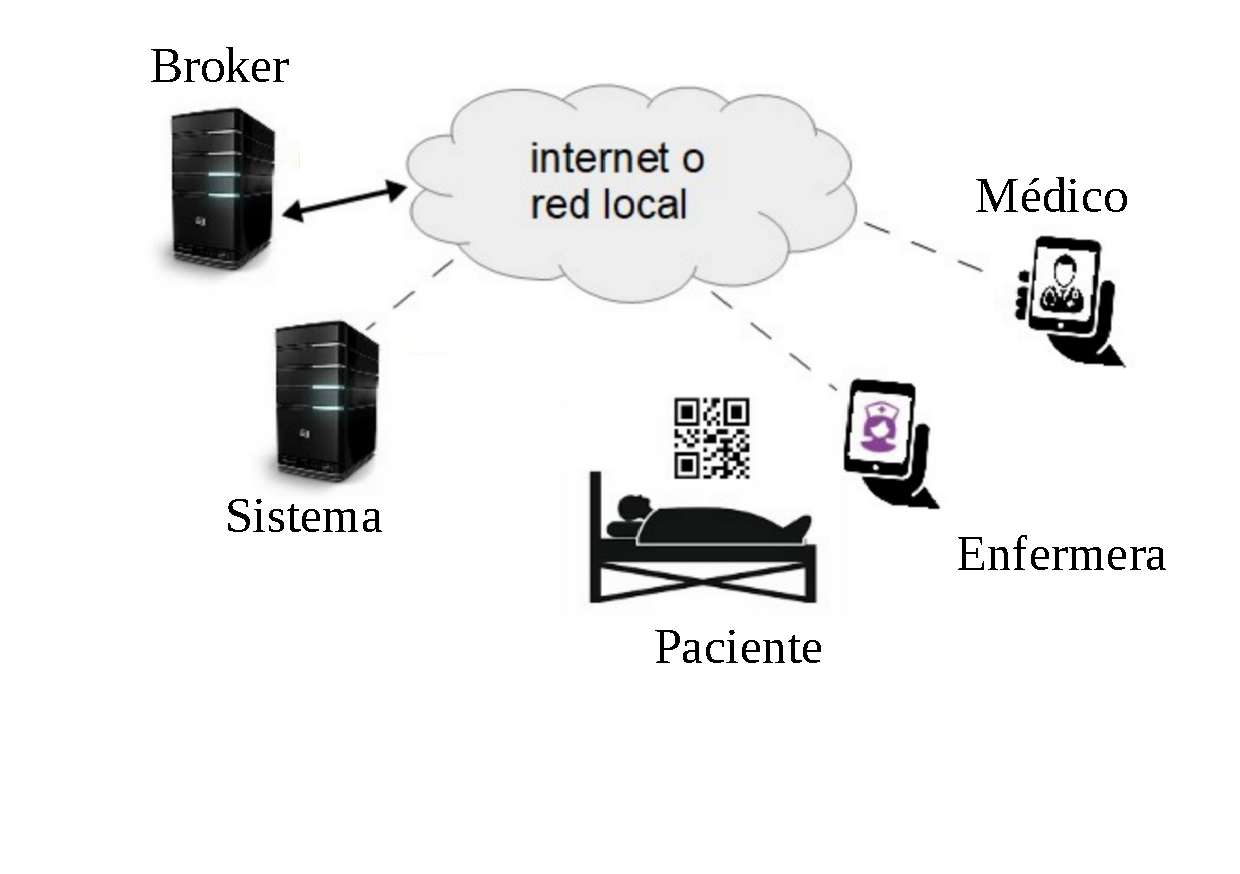
\includegraphics[width=.7\textwidth]{./Figuras/diag2.pdf}
\caption{ Diagrama en bloques del sistema.}
\label{fig:diagBloques}
\end{figure}

%\vspace{25px}

El broker recibe mensajes,llamados ``eventos'', de distintos publicadores y los reenvía a los subscriptores que correspondan según una política asignada previamente. El cliente sistema posee una base de datos con información relevante para los pacientes y tambien permite monitorear el estado de las habitaciones. Mientras que el cliente enfermera solo recibe asignaciones o respuestas de un médico, y publica finalización o consulta(por medio de una aplicación). Por último, el cliente médico solo recibe consulta y publica respuestas por medio de una aplicación.

Con la aplicacion web se puede cargar la base de datos con informacion de enfermeras, pacientes y médicos.
\vfill

 
%El tamaño de la tipografía en TODAS las figuras debe ser adecuado para que NO pase lo que ocurre acá, donde el lector debe esforzarse para poder leer el texto. Los colores usados en el diagrama deben ser adecuados, tal que ayuden a comprender mejor el diagrama, preferentemente en la gama de colores pastel.



\section{2. Identificación y análisis de los interesados}
\label{sec:interesados}


%Nota: (borrar esto y todas las consignas en color rojo antes de entregar este documento).
 
%Es inusual que una misma persona esté en más de un rol, incluso en proyectos chicos.
 
%Si se considera que una persona cumple dos o más roles, entonces sólo dejarla en el rol más importante. Por ejemplo:

%Pero en cambio sí es usual que el Cliente y el Auspiciante sean el mismo, por ejemplo.

\begin{table}[H]
%\caption{Identificación de los interesados}
%\label{tab:interesados}
\begin{tabularx}{\linewidth}{@{}|l|X|X|l|@{}}
\hline
\rowcolor[HTML]{C0C0C0} 
Rol           & Nombre y Apellido & Organización 	& Puesto 	\\ \hline
%Auspiciante   &                   &              	&        	\\ \hline
Cliente       & \clientename      &\empclientename	& Propietario       	\\ \hline
%Impulsor      &                   &              	&        	\\ \hline
Responsable   & \authorname       & FIUBA        	& Alumno 	\\ \hline
Colaboradores & --                   & --             	& --       	\\ \hline
Orientador    & \supname	      & \pertesupname 	& Director trabajo final \\ \hline
%Equipo        & miembro1 \newline 
%				miembro2          &              	&        	\\ \hline
%Opositores    &                   &              	&        	\\ \hline
Usuario final & Hospitales, personal de salud, administradores de sistemas         &  --            	&  --      	\\ \hline
\end{tabularx}
\end{table}

%El Director suele ser uno de los Orientadores.

%No dejar celdas vacías; si no hay nada que poner en una celda colocar un signo ``-''.

%No dejar filas vacías; si no hay nada que poner en una fila entonces eliminarla.

%Es deseable listar a continuación las principales características de cada interesado.
 
%Por ejemplo:
\begin{itemize}
%	\item Auspiciante: es riguroso y exigente con la rendición de gastos. Tener mucho cuidado con esto.
%	\item Equipo: Juan Perez, suele pedir licencia porque tiene un familiar con una enfermedad. Planificar considerando esto.
%	\item Orientador: María Gómez va a poder ayudar mucho con la definición de los requerimientos.
\item Orientador: Ericson va a poder ayudar mucho con la definición de los requerimientos.
\item Usuario final: Todos los usuarios del sistema como ser, administradores de redes hospitalarias, médicos y enfermeras, que deseen observar y/o controlar el proceso.

\end{itemize}





\section{3. Propósito del proyecto}
\label{sec:proposito}



El propósito de este proyecto es desarrollar un sistema para gestión de enfermeras basado en el protocolo MQTT compuesto por un broker, una web de configuración y una o varias aplicaciones, que agilice el desarrollo de funcionalidades futuras.
%¿Por qué se hace el proyecto? ¿Qué se quiere lograr? 

%Se recomienda que sea solo un párrafo que empiece diciendo ``El propósito de este proyecto es...''.


\section{4. Alcance del proyecto}
\label{sec:alcance}

{black}
%¿Qué se incluye y que no se incluye en este proyecto?

%Se refiere al trabajo a hacer para entregar el producto o resultado especificado. 

%Explicitar todo lo quede comprendido dentro del alcance del proyecto.

%Explicitar además todo lo que no quede incluido (``El presente proyecto no incluye...'')
El presente proyecto incluye:

\begin{itemize}
	\item Confección del plan de trabajo. 
	\item Investigación y estudio del protocolo MQTT, bases de datos SQL y NoSQL, programación de aplicaciones web y programación de aplicaciones multiplataforma.	
	\item Desarrollo local del broker que registre en un log actividades realizadas y su horario de realización. 
	\item Desarrollo local de una página web de configuración.
	\item Desarrollo local una de aplicacion cliente médico con envío/recepción de mensajes de audio/texto/alarmas.
	\item Desarrollo local una de aplicacion cliente enfermera con envío/recepción de mensajes de audio/texto/alarmas y escaneo de QR para identificar paciente. 
	\item Desarrollo local de una aplicacion cliente sistema que asigna enfermeras a pacientes adecuado a la indicación de un médico. Por ejemplo, todos los días a las 17 hs, medir la presión arterial del paciente "x", independientemente de la enferemera. Esta aplicación permite monitorizar el estado de las habitaciones.
	\item Documentación de las aplicaciones desarrolladas.

\end{itemize}

El presente proyecto NO incluye:
\begin{itemize}
	\item Manuales de las distintas aplicaciones desarrolladas.
	\item Traducciones a idiomas extranjeros de las aplicaciones y/o de la página web.
	\item Sistema llamador del paciente.
	\item Análisis en profundidad de tráfico en la red.
	\item Análisis en profundidad de Seguridad.
	\item Contratación de base de datos remota.
	\item Contratación e instalación de servidores remotos.
\end{itemize}



\section{5. Supuestos del proyecto}
\label{sec:supuestos}
Para el desarrollo del presente proyecto se supone que: 

\begin{itemize}
	\item Existe un llamador paciente. 
	\item Las aplicaciones moviles usaran iOS y Android como sistema operativo.
	\item La base de datos de los pacientes sólo puede ser afectada por medio de la aplicación sistema(el cliente médico sólo puede hacer consultas/modificaciones puntuales a una situación).	
	\item Se dispondrá al menos de una pc para instalación del servidor web, la base de datos, y del broker MQTT.
	\item Se dispondrá de un router para la prueba funcional del sistema. 

\end{itemize}

%\begin{consigna}{red}
%``Para el desarrollo del presente proyecto se supone que: ...''

%\begin{itemize}
%	\item Supuesto 1
%	\item Supuesto 2...
%\end{itemize}

%Por ejemplo, se podrían incluir supuestos respecto a disponibilidad de tiempo y recursos humanos y materiales, sobre la factibilidad técnica de distintos aspectos del proyecto, sobre otras cuestiones que sean necesarias para el éxito del proyecto como condiciones macroeconómicas o reglamentarias.
%\end{consigna}



\section{6. Requerimientos}
\label{sec:requerimientos}
Los principales requerimientos relevados son los siguientes:

\begin{enumerate}
	\item Requerimientos funcionales Servidor
			\begin{enumerate}
			\item El servidor debe tener instalado ECLIPSE MOSQUITTO como broker MQTT.
			\item El servidor debe tener funciones para interactuar con una aplicación Web, para consultas y envío de datos hacia dispositivos clientes.
			\item El servidor debe tener funciones para interactuar con la base de datos.
			\item El servidor debe proteger información del sistema.
			
			\end{enumerate}
	\item Requerimientos funcionales Base de datos
		\begin{enumerate}		
			\item El sistema debe poseer una base de datos relacional.
			\item La base de datos debe poseer datos cargados por default.
			\item La base de datos a utilizar debe poseer las siguientes tablas:
			
			*)Habitaciones
						
			*)Pacientes			
			
			*)Médicos
			
			*)Enfermeras			
			
			*)Eventos 

		\end{enumerate}	
	\item Requerimientos funcionales aplicación web de configuración
		\begin{enumerate}	
		\item La aplicación web debe ser cliente del broker MQTT.
		\item La aplicación web debe poseer funciones de consulta o modificación de la base de datos.
		\item La aplicación web debe ser permitir visualización de estadisticas de pacientes o enfermeras, etc.
		\item La aplicación debe de ser responsive.
		\item La aplicación debe contener acceso con usuario y contraseña para cada persona.
		\end{enumerate}			
	\item Requerimientos funcionales aplicación enfermera
		\begin{enumerate}
			\item La aplicación enfermera debe tener 3 modos de uso: usuario médico, usuario enfermera y usuario sistema.
			\item Al logearse el usuario (y contrastarse con la base de datos del sistema) se activa el modo correspondiente.
			\item La aplicación en modo enfermera debe permitir leer codigo QR.			
			\item La aplicación en modo enfermera debe poder descargar información relevante del paciente(medicamentos a suministrar, controles a realizar, contacto del médico a cargo del tratamiento,etc).	
			\item La aplicación en modo sistema debe mostrar las habitaciones sin atención,  según una tabla de prioridades(por ejemplo, si el mensaje es de algun dispositivo de urgencia-media), y en caso de igualdad de prioridades, la primera habitación que llamó.
			\item El modo usuario médico y el modo usuario enfermera deben poder enviar mensajes de textos o sonido comprimido en 32kbps(mp3).
			
		\end{enumerate}
	\item Requerimientos de documentación
		\begin{enumerate}
			\item Información de la base de datos: detalles de la misma y de API para acceder.
			\item Diagramas UML de aplicación sistema, aplicación enfermera, aplicación médico y página web.
			\item Información relevante para el uso del sistema.
		\end{enumerate}
	\item Requerimientos de integración de sistema:	
			\begin{enumerate}
			\item El sistema debe integrar el funcionamiento del servidor con base de datos y aplicación web.
			\item La aplicación web debe poder cargar la base de dato del sistema.
			\end{enumerate}	
	

\end{enumerate}


\section{7. Historias de usuarios (\textit{Product backlog})}
\label{sec:backlog}

%\begin{consigna}{red}
%Descripción: En esta sección se deben incluir las %historias de usuarios y su ponderación (\textit{history %points}). Recordar que las historias de usuarios son descripciones cortas y simples de una característica contada desde la perspectiva de la persona que desea la nueva capacidad, generalmente un usuario o cliente del sistema. La ponderación es un número entero que representa el tamaño de la historia comparada con otras historias de similar tipo.

%El formato propuesto es: "como [rol] quiero [tal cosa] para [tal otra cosa]."

%Se debe indicar explícitamente el criterio para calcular los \textit{story points} de cada historia
%\end{consigna}
\begin{itemize}
\item Como enfermero quiero que la aplicación me notifique si hay un pedido de una habitación para ir a atenderla.

Dificultad: baja(1) $\Rightarrow$ la notificación es solo un mensaje, y la existen varias formas de mostrarlo al usuario.

Complejidad: baja(1) $\Rightarrow$ tarea no sofisticada.

Riesgo: medio(3) $\Rightarrow$ puede haber situaciones de permisos que se desconocen al día de hoy.

Story Point: 5

\item Como enfermero quiero que la aplicación permita que notifique que finalicé la tarea para poder recibir otro pedido.

Dificultad: baja(1) $\Rightarrow$ la notificación es solo un mensaje.

Complejidad: baja(1)$\Rightarrow$ tarea no sofisticada desde el lado del enfermero.

Riesgo: medio(3) $\Rightarrow$ puede haber situaciones de permisos que se desconocen al día de hoy.

Story Point: 5

\item Como enfermero quiero que la aplicación permita que notifique que estoy atendiendo para que no tener varios pedidos pendiente.

Dificultad: media(3) $\Rightarrow$ el sistema gestor debe encontrar un mecanismo de monitoreo.

Complejidad: media(3) $\Rightarrow$ tarea no sofisticada desde el lado del enfermero, se resuelve desde el servidor.

Riesgo: bajo(1) $\Rightarrow$ es una tarea normal en sistemas statefull.

Story Point: 7

\item Como enfermero quiero que la aplicación permita que consulte a un médico para evitar cometer errores al tener dudas.

Dificultad: alta(5) $\Rightarrow$ se debe chequear la disponibilidad del médico de atenderlo, derivarlo a otro en caso contrario. Muchas opciones de mensajes y muchos test.

Complejidad: alta(5) $\Rightarrow$ Involucra prácticamente a todo el sistema.

Riesgo: alto(5) $\Rightarrow$ es la tarea principal del sistema y su complejidad puede escalar.

Story Point: 15


\item Como enfermero quiero que la aplicación permita obtener información del paciente para entender el estado de la situación.

Dificultad: media(3) $\Rightarrow$ se debe interconectar el cliente enfermera con la base de datos del servidor. Se debe presentar la información de manera clara en dispositivos con pantallas no muy amplias.

Complejidad: media(3) $\Rightarrow$  solo involucra al cliente enfermera y la base de datos.

Riesgo: bajo(1) $\Rightarrow$ el único riesgo que puede tener la tarea es la forma en que se presenta en el dispositivo, si la tarea contiene muchas líneas de texto puede que sea difícil de leer en un dispositivo móvil.


\item Como enfermero quiero que la aplicación permita avisar que mi jornada terminó para no recibir más notificaciones.

Dificultad: media(3)$\Rightarrow$ el sistema gestor debe encontrar un mecanismo de monitoreo.

Complejidad: media(3) $\Rightarrow$ tarea no sofisticada desde el lado del enfermero, se resuelve desde el servidor.

Riesgo: bajo(1)$\Rightarrow$ es una tarea normal en sistemas que mantienen un log de estado.

Story Point: 7


\item Como enfermero quiero que la aplicación permita que notifique que necesito ayuda de otro enfermero para atender el paciente.


Dificultad: alta(5) $\Rightarrow$ se debe chequear la disponibilidad de otro enfermero para atenderlo, derivarlo a otro en caso contrario. Muchas opciones de mensajes y muchos test.

Complejidad: alta(5) $\Rightarrow$ Involucra prácticamente a todo el sistema.

Riesgo: alto(5) $\Rightarrow$ su complejidad puede escalar

Story Point: 15

\item Como médico quiero que la aplicación posea un mecanismo sencillo para responder dudas de la enfermera.

Dificultad: baja(1) $\Rightarrow$ Se reutiliza el sistema del modo enfermera.

Complejidad: baja(1) $\Rightarrow$ Se reutiliza el sistema del modo enfermera.

Riesgo: bajo(1) $\Rightarrow$ Se reutiliza el sistema del modo enfermera.

Story Point: 3


\item Como médico quiero que la aplicación permita acceder a la información del paciente que en caso de consulta de un enfermero.

Dificultad: baja(1) $\Rightarrow$ Se reutiliza el sistema del modo enfermera.

Complejidad: baja(1) $\Rightarrow$ Se reutiliza el sistema del modo enfermera.

Riesgo: bajo(1) $\Rightarrow$ Se reutiliza el sistema del modo enfermera.


Story Point: 3


\item Como usuario sistema quiero que la aplicación me permita asignar tareas temporizadas para atender rutinas preestablecidas por el médico.

Dificultad: baja(1) $\Rightarrow$  tarea analoga a realizar un calendario con notificaciones. 

Complejidad: media(3) $\Rightarrow$ Se implementa en el lado servidor...multiples menues en la versión móvil(puede hacerse desde la página web también).

Riesgo: medio(3) $\Rightarrow$ Puede cambiar la forma de la presentación durante el desarrollo.


Story Point: 7


\item Como sistema quiero que la aplicación permita obtener datos estadísticos de cada enfermero para poder reportar.


Dificultad: media(3) $\Rightarrow$ Se gestiona desde la pagina web.

Complejidad: media(3) $\Rightarrow$ Se implementa en el lado servidor.

Riesgo: medio(3) $\Rightarrow$ Puede cambiar la forma de presentación durante el desarrollo.


Story Point: 9

\item Como sistema quiero que la aplicación móvil me muestre el estado de las habitaciones.

Dificultad: baja(1) $\Rightarrow$ Simplemente se almacenan los estados en la app o en el servidor.

Complejidad: baja(1) $\Rightarrow$ La implementación es bastante sencilla.

Riesgo: baja(1) $\Rightarrow$ Puede cambiar la forma de presentación durante el desarrollo.

Story Point: 3


\end{itemize}

\section{8. Entregables principales del proyecto}
\label{sec:entregables}



Los entregables del proyecto son :

\begin{itemize}
	\item Plan de Proyecto del Trabajo Final y Memoria Técnica
	\item Servidor MQTT 
	\item Base de datos configurada y con datos ficticios cargados
	\item Aplicación Web responsive
	\item Aplicación enfermera(con los 3 modos de funcionamiento)
	\item Integración de distintos sistemas.
	\item Código fuente de todo lo desarrollado.
\end{itemize}



\section{9. Desglose del trabajo en tareas}
\label{sec:wbs}


Desglose del trabajo:

\begin{enumerate}
\item Investigación preliminar( 60 hs)
	\begin{enumerate}
	\item Investigar funcionamiento Broker Mosquitto (10 hs)
	\item Investigar base de datos Relacionales(10 hs)
	\item Investigar bibliotecas graficas para implementar pagina web(20 hs)
	\item Investigar bibliotecas graficas para implementar aplicación movile(20 hs)
	\end{enumerate}
\item Implementación Servidor(110 hs)
	\begin{enumerate}
	\item Instalación y configuración de NodeJs como motor de ejecución de broker MQTT.(30 hs)
	\item Instalación de Broker MQTT (40 hs)
	\item Programación de funciones de consulta para aplicación web /movile (40 hs)

	\end{enumerate}
\item Implementación de la base de datos(110 horas)
	\begin{enumerate}
	\item Instalación de base de datos(40 horas)
	\item Configuración de parametros de seguridad y datos(30 horas)
	\item Creación y carga de datos ficticios para prueba(40 horas)

	\end{enumerate}
\item Implementación de página Web(190 horas)
	\begin{enumerate}
	\item Programación de funciones MQTT como cliente del broker(50 hs)
	\item Prueba de envío y recepción de datos al broker(10 hs)
	\item Programación de funciones de consulta de datos a la base de datos(40 hs)
	\item Programación de funciones de carga de datos a la base de datos(40 hs)
	\item Programación de logica y acceso de seguridad de usuarios(40 hs)
	\item Prueba de acceso de usuarios(10 hs)
	\end{enumerate}
	
\item Implementación de Aplicación enfermera(140 horas)
	\begin{enumerate}
	\item Programación de interface de usuario de logueo(4 hs)
	\item Programación de lógica y acceso de seguridad de usuarios(10 hs)
	\item Programación de interface de usuario modo enfermera(10 hs)
	\item Programación de interface de usuario modo médico(10 hs)
	\item Programación de interface de usuario modo sistema(10 hs)
	\item Prueba de envío y recepción de datos modo enfermera al broker(10 hs)
	\item Prueba de envío y recepción de datos modo médico al broker(10 hs)
	\item Programación de funciones de consulta de datos a la base de datos modo enfermera(10 hs)
	\item Prueba de envío y recepción de datos modo sistema al broker(10 hs)
	\item Prueba de envío y recepción de datos entre clientes modo enfermera y cliente modo médico (10 hs)
	\item Programación y prueba de lectura de QR usuario modo enfermera(6 hs)
	\item Programación y prueba de captura/compresión/envío de audio usuario modo enfermera(30 hs)
	\item Prueba de acceso de usuarios(10 hs)
	\end{enumerate}
\item Testeo de sistema(10 hs)
	\begin{enumerate}	
	\item Prueba del funciomiento correcto con 2 enfermeras 2 médicos y 3 llamadores  (10 hs)
	\end{enumerate}	
\end{enumerate}

Cantidad total de horas: (620 hs)



\section{10. Diagrama de Activity On Node}
\label{sec:AoN}

\begin{consigna}{red}
Armar el AoN a partir del WBS definido en la etapa anterior. 

%La figura \ref{fig:AoN} fue elaborada con el paquete latex tikz y pueden consultar la siguiente referencia \textit{online}:

%\url{https://www.overleaf.com/learn/latex/LaTeX_Graphics_using_TikZ:_A_Tutorial_for_Beginners_(Part_3)\%E2\%80\%94Creating_Flowcharts}

\end{consigna}

\begin{figure}[htpb]
\centering 
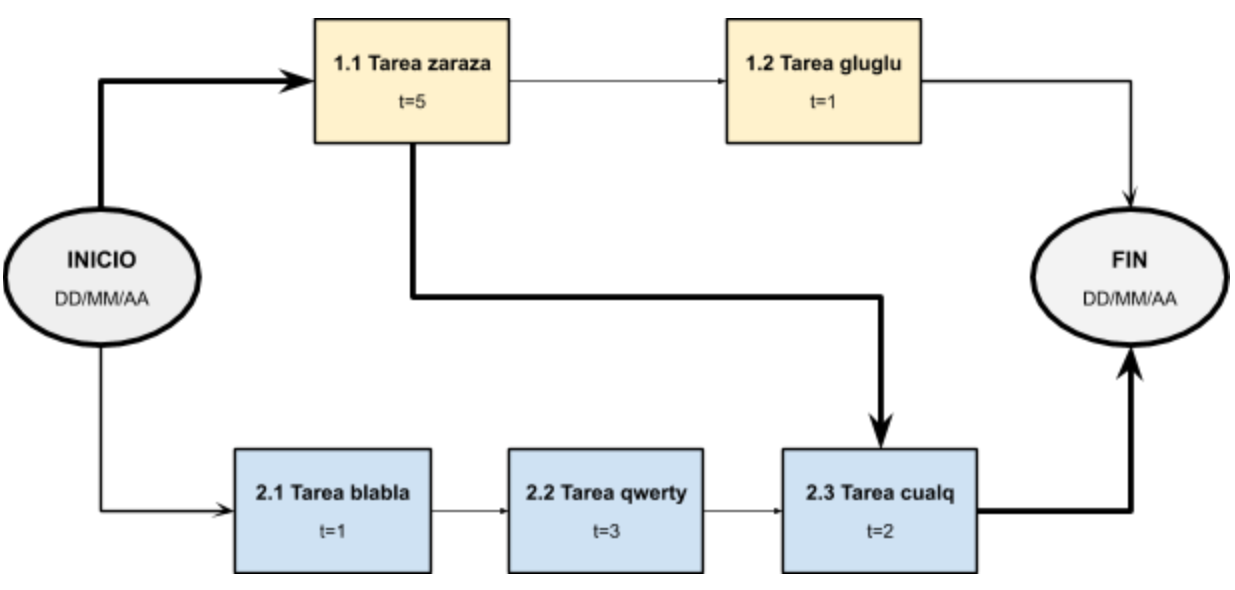
\includegraphics[width=.8\textwidth]{./Figuras/AoN.png}
\caption{Diagrama en \textit{Activity on Node}}
\label{fig:AoN}
\end{figure}

Indicar claramente en qué unidades están expresados los tiempos.
De ser necesario indicar los caminos semicríticos y analizar sus tiempos mediante un cuadro.
Es recomendable usar colores y un cuadro indicativo describiendo qué representa cada color, como se muestra en el siguiente ejemplo:



\section{11. Diagrama de Gantt}
\label{sec:gantt}

\begin{consigna}{red}

Existen muchos programas y recursos \textit{online} para hacer diagramas de gantt, entre los cuales destacamos:

\begin{itemize}
\item Planner
\item GanttProject
\item Trello + \textit{plugins}. En el siguiente link hay un tutorial oficial: \\ \url{https://blog.trello.com/es/diagrama-de-gantt-de-un-proyecto}
\item Creately, herramienta online colaborativa. \\\url{https://creately.com/diagram/example/ieb3p3ml/LaTeX}
\item Se puede hacer en latex con el paquete \textit{pgfgantt}\\ \url{http://ctan.dcc.uchile.cl/graphics/pgf/contrib/pgfgantt/pgfgantt.pdf}
\end{itemize}

Pegar acá una captura de pantalla del diagrama de Gantt, cuidando que la letra sea suficientemente grande como para ser legible. 
Si el diagrama queda demasiado ancho, se puede pegar primero la ``tabla'' del Gantt y luego pegar la parte del diagrama de barras del diagrama de Gantt.

Configurar el software para que en la parte de la tabla muestre los códigos del EDT (WBS).\\
Configurar el software para que al lado de cada barra muestre el nombre de cada tarea.\\
Revisar que la fecha de finalización coincida con lo indicado en el Acta Constitutiva.

En la figura \ref{fig:gantt}, se muestra un ejemplo de diagrama de gantt realizado con el paquete de \textit{pgfgantt}. En la plantilla pueden ver el código que lo genera y usarlo de base para construir el propio.

\begin{figure}[htbp]
\begin{center}
\begin{ganttchart}{1}{12}
  \gantttitle{2020}{12} \\
  \gantttitlelist{1,...,12}{1} \\
  \ganttgroup{Group 1}{1}{7} \\
  \ganttbar{Task 1}{1}{2} \\
  \ganttlinkedbar{Task 2}{3}{7} \ganttnewline
  \ganttmilestone{Milestone o hito}{7} \ganttnewline
  \ganttbar{Final Task}{8}{12}
  \ganttlink{elem2}{elem3}
  \ganttlink{elem3}{elem4}
\end{ganttchart}
\end{center}
\caption{Diagrama de gantt de ejemplo}
\label{fig:gantt}
\end{figure}


\begin{landscape}
\begin{figure}[htpb]
\centering 
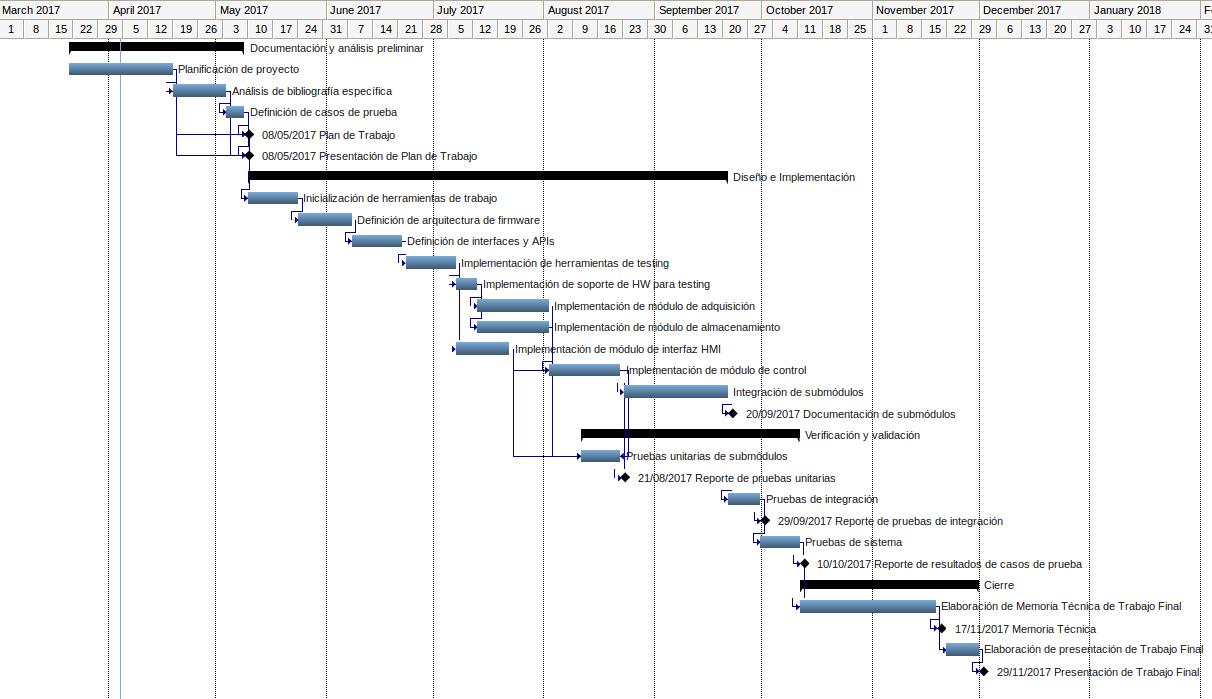
\includegraphics[height=.85\textheight]{./Figuras/Gantt-2.png}
\caption{Ejemplo de diagrama de Gantt rotado}
\label{fig:diagGantt}
\end{figure}

\end{landscape}

\end{consigna}


\section{12. Presupuesto detallado del proyecto}
\label{sec:presupuesto}

\begin{consigna}{red}
Si el proyecto es complejo entonces separarlo en partes:
\begin{itemize}
	\item Un total global, indicando el subtotal acumulado por cada una de las áreas.
	\item El desglose detallado del subtotal de cada una de las áreas.
\end{itemize}

IMPORTANTE: No olvidarse de considerar los COSTOS INDIRECTOS.

\end{consigna}

\begin{table}[htpb]
\centering
\begin{tabularx}{\linewidth}{@{}|X|c|r|r|@{}}
\hline
\rowcolor[HTML]{C0C0C0} 
\multicolumn{4}{|c|}{\cellcolor[HTML]{C0C0C0}COSTOS DIRECTOS} \\ \hline
\rowcolor[HTML]{C0C0C0} 
Descripción &
  \multicolumn{1}{c|}{\cellcolor[HTML]{C0C0C0}Cantidad} &
  \multicolumn{1}{c|}{\cellcolor[HTML]{C0C0C0}Valor unitario} &
  \multicolumn{1}{c|}{\cellcolor[HTML]{C0C0C0}Valor total} \\ \hline
 &
  \multicolumn{1}{c|}{} &
  \multicolumn{1}{c|}{} &
  \multicolumn{1}{c|}{} \\ \hline
 &
  \multicolumn{1}{c|}{} &
  \multicolumn{1}{c|}{} &
  \multicolumn{1}{c|}{} \\ \hline
\multicolumn{1}{|l|}{} &
   &
   &
   \\ \hline
\multicolumn{1}{|l|}{} &
   &
   &
   \\ \hline
\multicolumn{3}{|c|}{SUBTOTAL} &
  \multicolumn{1}{c|}{} \\ \hline
\rowcolor[HTML]{C0C0C0} 
\multicolumn{4}{|c|}{\cellcolor[HTML]{C0C0C0}COSTOS INDIRECTOS} \\ \hline
\rowcolor[HTML]{C0C0C0} 
Descripción &
  \multicolumn{1}{c|}{\cellcolor[HTML]{C0C0C0}Cantidad} &
  \multicolumn{1}{c|}{\cellcolor[HTML]{C0C0C0}Valor unitario} &
  \multicolumn{1}{c|}{\cellcolor[HTML]{C0C0C0}Valor total} \\ \hline
\multicolumn{1}{|l|}{} &
   &
   &
   \\ \hline
\multicolumn{1}{|l|}{} &
   &
   &
   \\ \hline
\multicolumn{1}{|l|}{} &
   &
   &
   \\ \hline
\multicolumn{3}{|c|}{SUBTOTAL} &
  \multicolumn{1}{c|}{} \\ \hline
\rowcolor[HTML]{C0C0C0}
\multicolumn{3}{|c|}{TOTAL} &
   \\ \hline
\end{tabularx}%
\end{table}


\section{13. Gestión de riesgos}
\label{sec:riesgos}

\begin{consigna}{red}
a) Identificación de los riesgos (al menos cinco) y estimación de sus consecuencias:
 
Riesgo 1: detallar el riesgo (riesgo es algo que si ocurre altera los planes previstos de forma negativa)
\begin{itemize}
	\item Severidad (S): mientras más severo, más alto es el número (usar números del 1 al 10).\\
	Justificar el motivo por el cual se asigna determinado número de severidad (S).
	\item Probabilidad de ocurrencia (O): mientras más probable, más alto es el número (usar del 1 al 10).\\
	Justificar el motivo por el cual se asigna determinado número de (O). 
\end{itemize}   

Riesgo 2:
\begin{itemize}
	\item Severidad (S): 
	\item Ocurrencia (O):
\end{itemize}

Riesgo 3:
\begin{itemize}
	\item Severidad (S): 
	\item Ocurrencia (O):
\end{itemize}


b) Tabla de gestión de riesgos:      (El RPN se calcula como RPN=SxO)

\begin{table}[htpb]
\centering
\begin{tabularx}{\linewidth}{@{}|X|c|c|c|c|c|c|@{}}
\hline
\rowcolor[HTML]{C0C0C0} 
Riesgo & S & O & RPN & S* & O* & RPN* \\ \hline
       &   &   &     &    &    &      \\ \hline
       &   &   &     &    &    &      \\ \hline
       &   &   &     &    &    &      \\ \hline
       &   &   &     &    &    &      \\ \hline
       &   &   &     &    &    &      \\ \hline
\end{tabularx}%
\end{table}

Criterio adoptado: 
Se tomarán medidas de mitigación en los riesgos cuyos números de RPN sean mayores a...

Nota: los valores marcados con (*) en la tabla corresponden luego de haber aplicado la mitigación.

c) Plan de mitigación de los riesgos que originalmente excedían el RPN máximo establecido:
 
Riesgo 1: plan de mitigación (si por el RPN fuera necesario elaborar un plan de mitigación).
  Nueva asignación de S y O, con su respectiva justificación:
  - Severidad (S): mientras más severo, más alto es el número (usar números del 1 al 10).
          Justificar el motivo por el cual se asigna determinado número de severidad (S).
  - Probabilidad de ocurrencia (O): mientras más probable, más alto es el número (usar del 1 al 10).
          Justificar el motivo por el cual se asigna determinado número de (O).

Riesgo 2: plan de mitigación (si por el RPN fuera necesario elaborar un plan de mitigación).
 
Riesgo 3: plan de mitigación (si por el RPN fuera necesario elaborar un plan de mitigación).

\end{consigna}


\section{14. Gestión de la calidad}
\label{sec:calidad}

\begin{consigna}{red}
Para cada uno de los requerimientos del proyecto indique:
\begin{itemize} 
\item Req \#1: copiar acá el requerimiento.

\begin{itemize}
	\item Verificación para confirmar si se cumplió con lo requerido antes de mostrar el sistema al cliente. Detallar 
	\item Validación con el cliente para confirmar que está de acuerdo en que se cumplió con lo requerido. Detallar  
\end{itemize}

\end{itemize}

Tener en cuenta que en este contexto se pueden mencionar simulaciones, cálculos, revisión de hojas de datos, consulta con expertos, mediciones, etc.  Las acciones de verificación suelen considerar al entregable como ``caja blanca'', es decir se conoce en profundidad su funcionamiento interno.  En cambio, las acciones de validación suelen considerar al entregable como ``caja negra'', es decir, que no se conocen los detalles de su funcionamiento interno.

\end{consigna}

\section{15. Procesos de cierre}    
\label{sec:cierre}

\begin{consigna}{red}
Establecer las pautas de trabajo para realizar una reunión final de evaluación del proyecto, tal que contemple las siguientes actividades:

\begin{itemize}
	\item Pautas de trabajo que se seguirán para analizar si se respetó el Plan de Proyecto original:
	 - Indicar quién se ocupará de hacer esto y cuál será el procedimiento a aplicar. 
	\item Identificación de las técnicas y procedimientos útiles e inútiles que se emplearon, y los problemas que surgieron y cómo se solucionaron:
	 - Indicar quién se ocupará de hacer esto y cuál será el procedimiento para dejar registro.
	\item Indicar quién organizará el acto de agradecimiento a todos los interesados, y en especial al equipo de trabajo y colaboradores:
	  - Indicar esto y quién financiará los gastos correspondientes.
\end{itemize}

\end{consigna}


\end{document}
